\secnumbersection{Definición del problema}

\subsection{Contexto}

Para realizar una simulación computarizada de un objeto, es necesario contar con una función capaz de describirlo. Cuando la geometría de éste es compleja, generalmente es imposible encontrar dicha función y es necesario aproximarla a través una composición basada en geometrías simples como hexaedros, primas, pirámides, etc. Esta aproximación mediante elementos geométricos recibe el nombre de malla geométrica.
% - Para realizar representaciones computacionales
% - Mallas geométricas
% - Octree 
% - Elementos básicos
% - Patrones de transición
% - Elementos inválidos y casos en los que se pueden generar.
\subsection{Mallas geométricas}

Una malla geométrica es una colección de elementos geométricos utilizados como representación computacional para el modelado tridimensional y/o animación.

Existen dos tipos de mallas geométricas, malla de superficie, que como dice su nombre representa sólo la superficie del dominio y donde los nodos internos no son utilizados, generalmente conformadas sólo por triángulos o paralelogramos, por otra parte, el otro tipo de malla es del tipo volumétrica, utilizada comúnmente para simulación, está compuesta generalmente por elementos geométricos volumétricos como tetraedros, hexaedros, prismas, etc. Este tipo de malla utiliza los nodos internos para análisis estructural, deformaciones, fracturas, el efecto del calor, entre otras.

% Existen dos diferentes estructuras de las que se pueden constituir una malla geométrica, fijas o adaptativas, una malla fija es la que se construye según un patrón predeterminado, por ejemplo, una malla uniforme conformada de solamente cuadrados de diferentes tamaños y distribuidas de tal forma que cubran todo el dominio. En cambio, una malla adaptativa se construye en función del contenido del dominio.  
En ciertas aplicaciones de mallas geométricas como por ejemplo en el contexto de simulaciones biomédicas, como la técnica usada en \cite{lobos2015mixed} para mallados en tiempo real en el ámbito biomédico, se requiere realizar un acercamiento a una o más zonas del objeto simulado a estudiar, este proceso se le denomina refinamiento.

En esta memoria se utilizará la técnica Octree con elementos mixtos, malla Octree mixta, para representar y refinar las mallas geométricas volumétricas.

\subsection{Mallas Octree mixtas}

La técnica Octree es una de las más utilizadas para concentrar nodos en una región determinada de una malla. 
Cada nodo de un Octree se denomina octante. La idea básica consiste en dividir un octante en varios octantes nuevos de forma recursiva.

El octante es una estructura en árbol de datos en la que cada nodo de este se divide en un número constante de nodos hijos, normalmente en 8 o 27 hexaedros, estos nodos serán los encargados de generar figuras geométricas como hexaedros, prismas, pirámides y tetraedros que son mostradas en la Fig. \ref{fig:basics_elements}.
Cuando se utiliza la división en 27, es posible generar una malla hexaédrica pura. Sin embargo, cuando se utiliza el proceso 8-split, las transiciones entre regiones finas y gruesas sólo pueden gestionarse introduciendo diferentes tipos de elementos, a esto se le denomina malla octree mixta.

\begin{figure}[h]
    \centering
    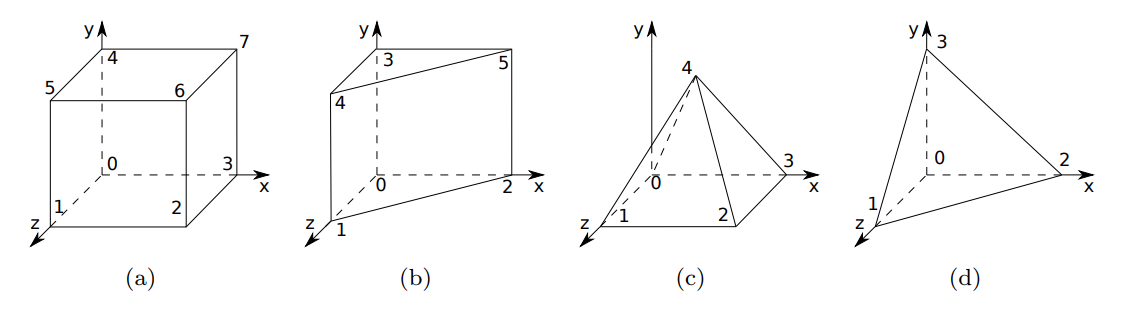
\includegraphics[width=0.95\textwidth]{figures/basic-elements.png}
    \caption{\label{fig:basics_elements} Elementos básicos}
     \small{(a) hexaedro, (b) prisma (cuña), (c) pirámide y (d) tetraedro.} \\
    Fuente: \cite{Gonzalez2014}
\end{figure}

% proceso de division en octantes
Supongamos que $\Omega$ es el dominio de entrada para el que se requiere generar una malla. La mayoría de algoritmos de mallado basados en octantes encapsulan el dominio $\Omega$ en un octante principal o primario y, a continuación, proceden a subdividir recursivamente los octantes hasta que se cumple una determinada restricción, generalmente un delta de error de representación.

El número de subdivisiones recursivas realizadas sobre un octante se denomina nivel de refinamiento ($RL$). Algunos algoritmos ofrecen la posibilidad de definir distintas regiones de refinamiento sobre $\Omega$. Para cada región, puede definirse un $RL$ mínimo y un octante puede pertenecer a varias regiones. Cuando un octante se divide y algunos de sus hijos se sitúan completamente fuera del dominio $\Omega$, su proceso de refinamiento se detiene y se eliminan de la representación.

Un octree equilibrado significa que dos octantes adyacentes no pueden tener una diferencia de nivel de refinamiento superior a uno, como se menciona en \cite{daines2018repairing}. Una malla basada en octantes suele requerir un octree de este tipo. Para ello, algunos octantes se refinan más allá de su $RL$ original. En la Fig.\ref{fig:octree-mesh} se muestra un ejemplo análogo en 2D para ilustrar el proceso de división en 8 hexaedros.

La tarea principal de esta investigación es el refinamiento de las mallas, es decir, aumentar la densidad de nodos que conforman la malla para así aumentar a su vez la definición de la representación. Sin embargo este aumento en la cantidad de nodos no debe ser uniforme en toda la malla ya que afectaría considerablemente el tiempo de ejecución de las simulaciones. Es por esto que algunas técnicas de generación de mallas utilizan refinamiento parcial \cite{lobos2015mixed}, donde son seleccionadas ciertas regiones de la malla en las que se quiere mayor definición y solo dichas zonas de interés son refinadas. En el caso de la figura \ref{fig:octree-mesh}, una malla en 2D de refinamiento parcial, la región de interés es el borde del dominio identificado con el color gris.

\begin{figure}[!ht]
    \centering
    % 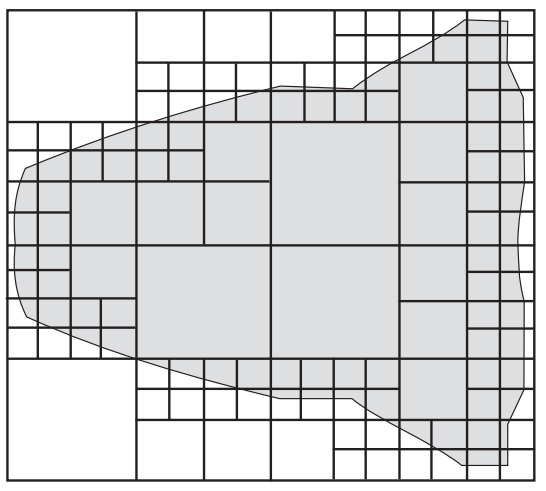
\includegraphics[width=0.5\textwidth]{figures/octree-mesh.png}
    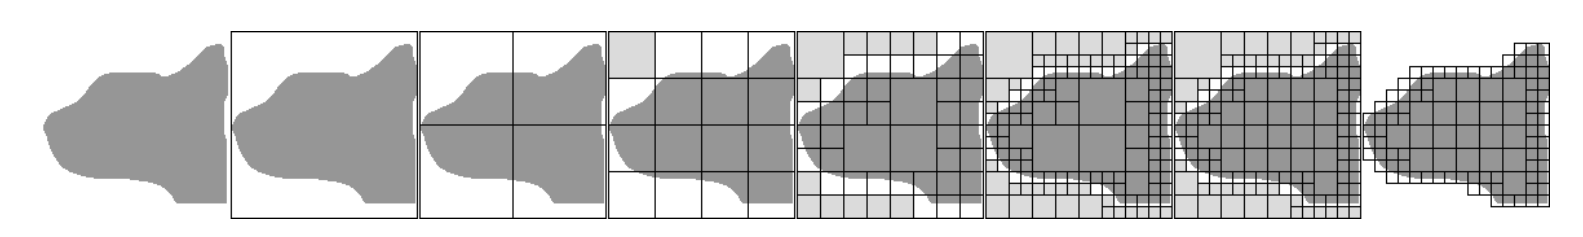
\includegraphics[width=1.0\textwidth]{figures/divison-process.png}
    \caption{\label{fig:octree-mesh} Malla Octree parcialmente refinada.}
    \small{Ejemplo en 2D de la generación de una malla octree equilibrada utilizando un algoritmo basado en Octree.
    Con nivel de refinamiento $RL$ 4 en la región $\Omega$ demarcada con gris. El resto de la malla no tiene definido un $RL$ mínimo, por lo que los octantes que no intersectan con el límite de $\Omega$ tienen su refinamiento detenido.} \\
    Fuente: \cite{lobos2015mixed}
\end{figure}

En una malla al haber distintos niveles de refinamiento, se pueden formar mallas no conformes. 

Un octree equilibrado no es conforme cuando hay múltiples $RL$ y no se respeta la regla de los $RL$ adyacentes. Para mantener la continuidad de la malla, debe aplicarse un patrón de transición sobre los octantes con vecinos de diferentes $RL$. Un patrón de transición sustituirá el hexaedro no conforme por diferentes tipos de elementos, de modo que se garantice que la malla de salida sea conforme. En la Fig. \ref{fig:transition_pattern}  se muestra un ejemplo de patrón de transición.

Una malla es conforme cuando es topológicamente correcta, es decir, tiene todos sus nodos de los bordes y caras consistentes para todos los elementos adyacentes. 

Para construir una malla conforme con refinamiento parcial, se puede hacer uso de elementos especiales que forman transiciones entre regiones con distinto nivel de refinamiento. Este conjunto de elementos se le denomina patrones de transición. En la Fig. \ref{fig:transition_pattern} se puede observar que el elemento B constituye un patrón de transición entre zonas con distinto nivel de refinamiento, en donde el elemento A presenta más refinamiento que el elemento C.

\begin{figure}[!ht]
    \centering
    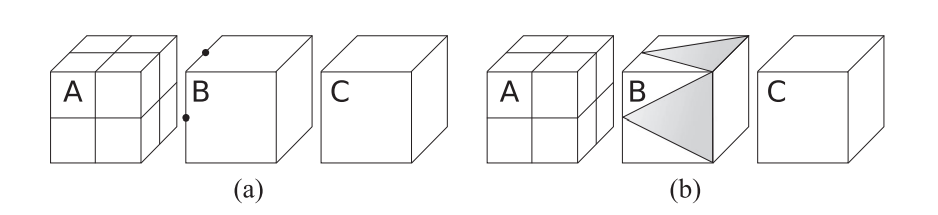
\includegraphics[width=1\textwidth]{figures/transition_pattern_complete.png}
    \caption{\label{fig:transition_pattern} Patrón de transición.} 
    \small{(a) Octante B es el único elemento que requiere un patrón de transición. (b) Malla conforme, topológicamente correcta, resultante de la transición.} \\ Fuente: \cite{lobos2015mixed}.
\end{figure}

La técnica de generación de mallas a utilizar en esta memoria será la técnica que utiliza elementos mixtos para construir patrones de transición.
Dichos elementos son tetraedros, hexaedros, prismas y pirámides de base cuadrada. Todos los patrones existentes fueron diseñados y presentados en \cite{Gonzalez2014}. Además, también hay técnicas que los utilizan para la representación de los bordes en la malla, definiendo un conjunto de elementos, llamados patrones de superficie, que reemplazan los hexaedros encontrados en los bordes.

Algunas mallas de refinamiento parcial pueden verse afectadas negativamente por transiciones entre regiones de diferente nivel de refinamiento en la superficie, llegando muchas veces a invalidar ciertos elementos involucrados. 

% explicación de invalidación
% imagen de elementos invalidados

Aquí se evidencia que los patrones de superficie para generar estas transiciones no están diseñados para ser aplicados sobre elementos mixtos, sino que solamente para mallas compuestas por hexaedros.  Esto puede surgir especialmente en sectores de la malla donde el dominio es cóncavo. 

\subsection{Actualidad}

Actualmente existe un estudio \cite{daines2018repairing} que consiste en reparar elementos inválidos en la superficie de mallas tipo Octree con elementos mixtos y refinamiento parcial. En este estudio se propone una técnica de proyección de nodos para reparar aquellos elementos de los bordes en regiones de transición de la malla, esta técnica se aplica iterativamente debido a que en cada iteración se pueden generar nuevos elementos inválidos.

\subsection{Lineamiento}


% por qué es importante la calidad de los elementos
% cómo se medirá la calidad
% qué es validar la malla
% por qué es importante validar la malla

Se desarrollará desde otra perspectiva la reparación de los elementos inválidos en las regiones de transición que pueden generarse al intentar lograr una representación correcta de los límites.



\subsection{Objetivos}
\subsubsection{Objetivo general}
Ubicar y reparar elementos inválidos o de mala calidad en la superficie de una malla geométrica tridimensional de tipo octree.

\subsubsection{Objetivos específicos}
\begin{itemize}
    \item Validar la malla resultante de la refinación mediante la técnica Octree.
    \item Medir la calidad de la malla generada y refinar los elementos que sean inválidos.
    \item Establecer una estructura de datos que permita volver a un estado anterior de la malla, así en caso de que existan elementos inválidos, permitir volver a un estado válido anterior.
    \item Realizar pruebas para posteriormente comparar tiempos de ejecución con respecto a la versión propuesta en \cite{daines2018repairing}.
\end{itemize}

% Se debe definir el problema, es importante no confundir definir el problema con describir la solución. Por ejemplo: ``diseñar una arquitectura e implementar una plataforma ...'' es una solución, no un problema.

% Algunos elementos que podrían ir en este capítulo son (no es necesario que vayan todos):
% \begin{itemize}
%     \item Breve descripción del contexto donde se realizará la memoria (organización, línea dentro de la Informática en la que se basa, etc.)
%     \item ¿Qué y cómo se realiza actualmente la situación que mejorarás con tu memoria?
%     \item ¿Qué actores o usuarios están involucrados?
%     \item ¿Qué dificultades tienen esos actores actualmente? ¿cuántos son? (ideal si se pueden poner estadísticas para así saber si existe un mercado razonable para la solución que propondrás en tu memoria, en el fondo saber cuántas personas u organizaciones tienen el mismo problema que estás definiendo)
%     \item ¿Qué podría pasar si en el corto o mediano plazo no se solucionan esas dificultades (¿es decir, si no se hiciera tu memoria, qué pasaría?; en el fondo justificar por qué conviene hacer tu memoria, ¿cuál es la motivación o interés de hacerla?).
%     \item ¿Qué competencia existe actualmente? (a lo mejor ya existe una solución al problema, pero por qué no sirve, o por qué tu solución sería mejor, también se puede enfocar a si este problema existe en otras realidades y cómo ha sido solucionado allí).
%     \item Precisar los objetivos y alcances de la memoria (o solución al problema).
% \end{itemize}

% En este capítulo, de ser necesario puede usar referencias bibliográficas (velar porque sean recientes), una cita de ejemplo \cite{schwab2002cure} y otras más \cite{georget1994study,beaumont1990patient}.

% Recuerde poner notas al pie de página que sean explicativas \footnote{Este es un ejemplo de una nota al pie de página. Puede indicar alguna URL, definiciones, aclarar alguna información pertinente del texto, citar algunas referencias, etc..}.
